\documentclass{article}
\usepackage[T1]{fontenc}
\usepackage{lmodern}
\usepackage{graphicx}
\usepackage{amsmath,amssymb}
\usepackage[a4paper,margin=2cm]{geometry}
\usepackage[absolute,overlay]{textpos}
\setlength{\TPHorizModule}{1mm}
\setlength{\TPVertModule}{1mm}
\usepackage[indonesian]{babel}
\usepackage{hyperref}
\setlength{\emergencystretch}{2em}
% unit: Halaman 12

\begin{document}

% === Halaman 12 (llm) ===

\vspace{68.31mm}

\section*{Ancient Steganography}

\begin{itemize}
    \item \textbf{Steganografi dengan media kepala budak.}
\end{itemize}

Ditulis oleh Herodotus ($485 - 525$ BC), sejarawan Yunani pada tahun $440$ BC di dalam buku: \textit{Histories of Herodotus}. Kisah perang antara kerajaan Persia dan rakyat Yunani.

\vspace{10mm}

Herodotus menceritakan cara \textbf{Histaiaeus} mengirim pesan kepada \textbf{Aristagoras of Miletus} untuk melawan Persia. Caranya: Dipilih beberapa budak. Kepala budak dibotaki, ditulisi pesan dengan cara tato, rambut budak dibiarkan tumbuh, budak dikirim. Di tempat penerima kepala budak digunduli agar pesan bisa dibaca.

% deskripsi: Potret Herodotus
% bbox normalisasi: [0.8800, 0.0100, 0.9770, 0.2400]
\begin{textblock*}{20.37mm}(184.80mm,2.97mm)
\noindent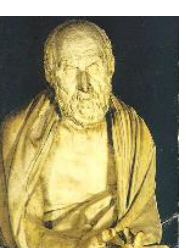
\includegraphics[width=20.37mm,height=68.31mm]{../../images/llm/page_012_img_01.png}%
\end{textblock*}

% deskripsi: Ilustrasi proses steganografi pada kepala: tato pesan, penumbuhan rambut, dan pencukuran kembali untuk membaca pesan
% bbox normalisasi: [0.1600, 0.7000, 0.8500, 0.9500]
\begin{textblock*}{144.90mm}(33.60mm,207.90mm)
\noindent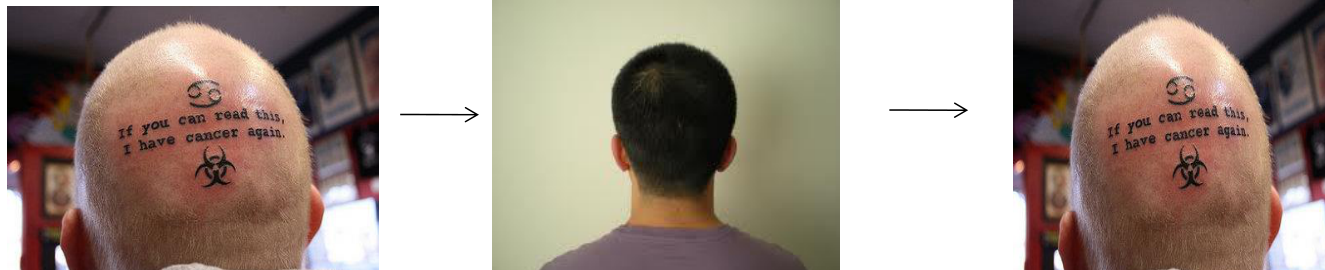
\includegraphics[width=144.90mm,height=74.25mm]{../../images/llm/page_012_img_02.png}%
\end{textblock*}

\end{document}
